\newpage
\section{NOSQL (Not Only SQL)}


% Introduzione
\subsection{Introduzione}

Sono dei \hl{database distributi} con:

\begin{itemize}
    \item storage semistrutturato
    \item alta replicazione dei dati
    \item alte prestazioni
\end{itemize}

Non sarà richiesto uno schema ER, e ha come \hl{tipi}:

\begin{itemize}
    \item documentali
    \item chiave valore
    \item colonnari
    \item a grafo
    \item ibridi
    \item a oggetti
    \item xml
\end{itemize}


% CAP Theorem
\subsection{CAP Theorem}

Se ho modelli diversi di DB vorrei poter avere \hl{diversi livelli di consistenza dello stato del DB} e voler forzare la transazione. Allora dovremo avere:

\begin{itemize}
    \item \hl{consistenza}: in tutti i DB distribuiti \textbf{ciscuna istanza deve fornire gli stessi dati}
    \item \hl{disponibilita'}: \textbf{un fail del nodo master non deve intaccare gli altri}
    

    \begin{figure}[H]
    \centering
    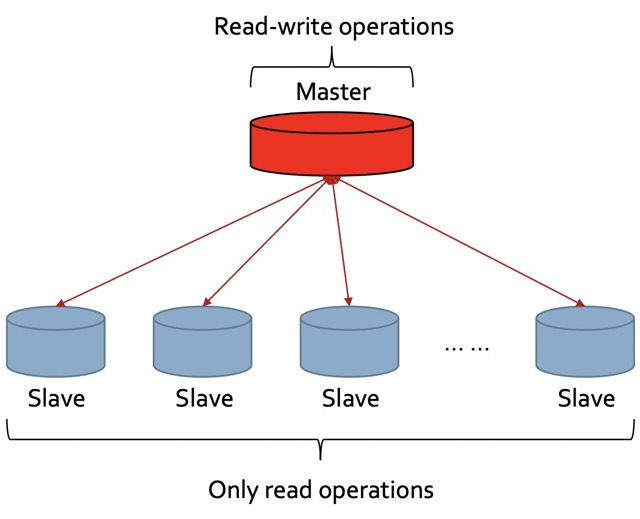
\includegraphics[scale=0.4]{masterslave.jpeg}
    \caption{Master and sleave} 
    \label{masterslave}
    \end{figure}


    \item \hl{partizione}: il sistema continua a \textbf{funzionare nonostante la perdita di messaggi, o problemi di connessione}
\end{itemize}

Se ho un sistema distribuito \hl{non possono garatire tutte e 3 le cose}, allora possono essere garantite \hl{solo 2 alla volta}:

\begin{figure}[H]
\centering
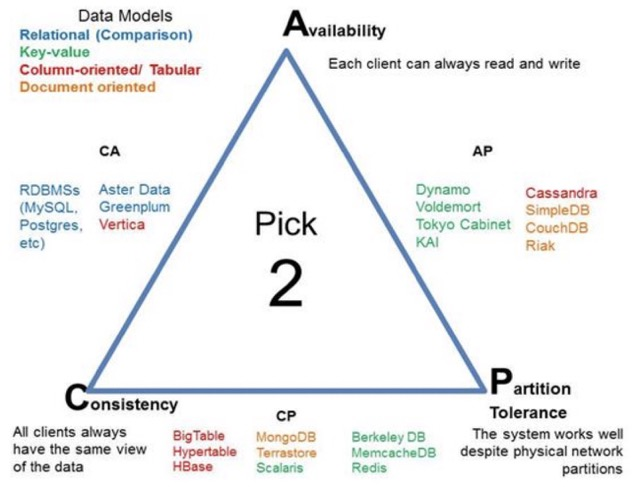
\includegraphics[scale=0.4]{cap.jpeg}
\caption{CAP theorem} 
\label{cap}
\end{figure}


tutto questo vale solo se il DB è distribuito.

Le combinaiozni sono:
- CA: non soddisfatta la partition tollerance, cioe1 che quella funzione viene meno per qualche motivo posso allora avere dei piccoli sistemi che non devono indertagire ed altre che dovrebbero non possono. ci sono allora i dbms che in assenza di comunicazione garantiscono consistenza e disponibilita
- CP: non soddisfa la disponibilita1 e quindi se non devo garantire la disponibilita allora ad un isstemsta e1 consetito di non rispondere a tutte le richeiste in lettura e scrittura, in pratica vincola la transazione dato che sacrififcanos la disponibilita nela transazione npn posso leggere i dati 
- AP: perdo la consistenza, quindi all'istante t i pari client possono vedere dati diversi, ogni parte del sistema fa vaedere i dati ai quali ha accesso. Allora non e1 garantito che in qualsiasi istante tutte le aprtizioni grataniscno la stessa vista sugli stessi dati

riportare consequence of cap

l'idea ala base del CAP theorem cdel poter avere solo 2 punti ora come ora e1 meno importante perceh se ho poche partizioni non e1 importante perdere Co A se il sistema non e1 partizionato (cosa che succedeva prika,a) oopure si verifica ceh scegliere tra C e A si verifica piu volte infatti il sistema e1 portato da richieste  tante richeiste dato ceh succede ceh C o A possono essere richieste insieme tante volte per ogni interazione allora bisogna sempre switcahre 


per mettere insieme queste idee inseme: vado a pefinire a priori delle casistiche nele quali una delle 3 caratteristiche viene sacartata (il porgettita lo fa)



BASE: conseguenza del cap teheorem che al posto di vincolarmi ai 3 vertici del triangolo faccio n trade-offe trovo non una perfetta dispoinibilita dei 2 punti ma una buona di base:
basically available:
soft state: dico che volgi oi dati consistenti solo alla fine e non per forza in ogni istante alora devo assicurarmi che al sistema no narrivino altri input qunado sto craeando la consistenza
softstate ????

vedere slide torino

ACID: focus sulla consistenza ...
BASE: alta disponibilita al posto di consistenza assoluto, quindi garantiere scrittura e lettura semrep








non0relational databases for data managment:
dividon in piccole unita le mie strutture dati allora la struttura la conosco in anticipo dato che ho fatto pirma concettuael poi logico e pi i lfiscio 
... slide 5


quidi se volgio garantier ele join tra le trabelle e tle transazioni ho bisogno di un dsistema centralizzato. posso allora pensare a quei casi in cui voglio rilassare alcunidi queti vincoli.

ne rientrano i no qsl

1. tenere in sieme fisiicamente nellastessa partizoini i dati che saranno acceduti insieme
2. garanzia che la lettura sia piu rapida
3. rilassare la resistenza che sara1 locale 
4. il modello dati  dei db puo variare e son o4" chiave valore, documento, colonnale, grafo

dove i pirami 3 sono basati su aggregaione


caratteristiche\;
non mi servono le join
no schemi
garantisce la scalabilita orizzontale


confronto:
ralazionali / non relazionali
- ogni record ha una riga / soluzione diversa per ogni dbms
- sceham predefinito per ognitabela con scambio costoso dato ceh devo fermare tutto / schema dinamico cosi non devo per forza acccedere ai campi per come sono stati srcitti
- scalaboilita verticale: per aumentare le prestazionei del db deviaumetntare le capacita dell'hardware (aumento la potenza dle singolo server / piu volgio aumentare le prestazioni piu aumento i nodi (server) 
- ogniuno ha un suo linguaggio di query / custom query focus sulle collection dei documenti
- serve per dati piatti dove conosco la struttura / per dati gerarchici con file json o xml con un nodo radice e delle diramazioni


relazionane ha tutte le cAP quando lo distribuisco perdo la P(aggiungere su)


pro dei nosql:
- vanno beene per dati semistrutturati o gerarchici
- in quali sistuaizoni: applicazionie online (per i file json ecc)
- se voglio incrementare le prestazione delle query in parallelo ed avere dati ridondanti
- alto livello di accesso concorrente
- molte letture e scritture
- letture e scrittura consistenti

contro:
- a linelo di transazioni consistenza non sepre garantita
- datio denjormalizzati, cioe collegati con piu colegamenti tra loro, allora dobbiamo accedere a piu dati rispetto al ralzzionale
- no chiavi esterne
- caso di aggiornamento di molti dati questo sara molto lento (scrievere o modificatre dati quindi) e serve piu stazio fisico + 10/50 volte del relazionele
- se decido di cambiare la struttura non riesco a tracciarli facilemte dato ceh no c'e il cpncetto di schema


si usa perche1 
1. le grandi software house le usano
2. in alcunie situaizoni il vantaggio e1 oggettivo : in quelle in cui posso sfruttare
- buona scalabilit (piu server)
- gestire scehmi diversi
- leggere rapidamente(azioni web)
- non serve pompare il server e qindi funzionano anche su hardare anceh che non cosano troppo


challeges of nosql:
1. tecnologia non troppo matura dato che esiset da -20 anni
2. no supporto all'utenza ma ci son ole community
3. a parte di amministrzione e1 piu difficile 
4. mancano degli standard tra i vari nosql


img slide 23

chiave valore: ad ogni chiave e1 associato un solo valore
cononnale: ad ogni chiave sono associati piu valori, ma le colonne non hanno dei conecetti valori 
documentale: albero binario 
grafo: posso andare ovunquwe infatti e1 orienteato e possiamo decidere se dargli un verso di percorrenza



documentale: si basa sul concetto di aggregazione e basato su un sieme di coppie chiave valore, allora un documento sara un aggrergazione di isatnze di coppie chiave valoreci accedo a queste aggregazioni in base ai campi che ho.
ogni documento e1 un sisnsieme di dati autoconsistente. non ho dati sparpagliati n varie trabelle.


mongodb: CP

gerarchia:

fig slide 21


relational / mongodb
database / database
tavle, view / collection
row /document BSON
comun / field
index / index
join / embedded document
foreing key / reference al documento che server
partition / shard

mongodb -> database instance
mongos -> sharding process

aggreghiamo in una stessa collection dei documenti che per l'implementatore hanno senso

per effettuare delle operazioni:
db.collection_name.operatoion

create operation:
save, update, insert

read operation:
find=SELECT, 
